\newpage
\section{Analyse des besoins fonctionnels}
\label{besoins:fonc}

\subsection{Génération de Playlist}
\label{besoins:fonc:generation}

L’objectif principal de ce projet est de générer une liste cohérente de morceaux
selon des paramètres choisis par l’utilisateur. Cette génération se décompose en 2 parties distinctes.

\subsubsection{Sélection: interaction avec les données}
\label{besoins:fonc:generation:selection}

Durant l’étape de sélection, le programme doit être capable de choisir un ensembles
morceaux correspondant à un certain nombre de critères, tous étant optionnels, cette ensemble s'appelle la Pool de morceaux.
Dans le cas où aucun des paramètres optionnels n’est fixé, les pistes
sélectionnées doivent êtres aléatoires.

\vspace{3mm}
\noindent Les paramètres sont les suivants~:
\begin{itemize}
\item Durée de la playlist en temps ou en nombre de morceaux.
\item Le nom d'un artiste
\item Un tranche d'années
\item Un score de popularité
\end{itemize}

\vspace{3mm}
\noindent À ces données, on ajoute trois données basées sur le signal~:
\begin{description}
\item[Rythme~:] tout d’abord calculée d’après le tempo.
\item[Énergie~:] pouvant être calculée à partir du paramètre de «~loudness~».
\item[Humeur~:] pouvant être calculée en fonction de la tonalité du morceau (Note~: l’humeur
n’est pas nécessairement une donnée basée sur le signal, le client peut très bien
donner cette information en recueillant des avis d’utilisateurs).
\end{description}

Ces informations sont considérées exactes dans la base de données, elle sont toutes stockées dans des nombres flottant allant de 0 à 1, libre au créateur d'un nouvelle base de données d'imposer sa convention pour le calcul de ces valeurs.

\subsubsection{Ordonnancement: Similarité entre les morceaux}
\label{besoins:fonc:generation:selection:ordonnancement}

Durant l'ordonnancement, les morceaux placés dans la Pool de morceaux doivent être agencés en respectant une cohérence, mais aussi une variété. Un score de similarité doit donc pouvoir être calculé entre les morceaux pour choisir celui qui convient le mieux.

Ce calcul de similarité doit pouvoir donner un score de similarité entre 2 morceaux. Une playlist cohérente est donc une playlist dans laquelle chaque morceau doit avoir un score de similarité élevé avec le morceau qui le précède.

\subsection{Visualisation de la playlist}
\label{besoins:fonc:generation:visu}

La playlist doit pouvoir être utilisable après avoir été générée. IL faut donc un
moyen de la visualiser, et possiblement, de l’écouter.
Le moyen le plus simple, mais le plus rustique est le format textuel. Ce format
de sortie sera requis principalement pour les tests, son utilité est réduite dans
les autres cas.

Un autre moyen de visualiser la playlist est d’utiliser un service de streaming.
Celui qui a retenu notre attention est Deezer, car son API est en accès libre et
que la construction de playlist est assez simple. Il suffit en effet d’utiliser
une API javascript.
        
\subsection{Interface Utilisateur et feedback}
\label{besoins:fonc:generation:feedback}

Pour interagir avec le générateur, l’utilisateur doit passer par une interface
utilisateur (graphique ou en console) permettant de paramétrer le dit générateur.
De plus, dans le cas de certaines interfaces utilisateurs, il est important
d’envoyer un feedback des actions réalisées par le programme à l’utilisateur. Il
faudra donc utiliser un système nous permettant de visualiser l’avancement de la
génération.

\newpage

\section{Analyse des besoins non fonctionnels}
\label{besoins:nfonc}

\subsection{Performances}
\label{besoins:nfonc:perf}

Les performances de la génération de la playlist sont importantes, car nous
voulons éviter de frustrer les utilisateurs avec un temps d'attente trop long.

Le feedback de l’interface permettra de réduire cette frustration, mais il faut
aussi raisonner en performance brute. Le nombre de pistes correspondants aux
critères rentrés par l’utilisateur peut être énorme. Il faut donc filtrer et
limiter le nombre de ces résultats, tout en conservant une notion d’aléatoire.

Nous avons donc décidé de limiter le nombre de morceaux sur lesquels faire nos
calculs et notre ordonnancement, les morceaux sélectionnés étant un sous ensemble
plus petit des morceaux correspondant aux critères choisis. Notre convention est
donc de limiter ce sous ensemble de pré-sélection à 10 fois la taille de playlist
demandée par l’utilisateur, ainsi pour une génération de 15 morceaux, une préselection de 150 morceaux sera faite et la génération sera effectuée depuis uniquement ces morceaux.

\subsection{Modularité}
\label{besoins:nfonc:perf:mod}
    
Le projet se doit de pouvoir avoir chacune de ses parties indépendantes et
remplaçables à souhait. Pour cela, le programme sera séparé en 4 modules~:

\subsubsection{Module d'Interface Utlisateur}
\label{besoins:nfonc:perf:mod:iu}

(c.f. Section \ref{sec:interface})

\subsubsection{Module de génération de playlist}
\label{besoins:nfonc:perf:mod:generator}

Le module est chargé de générer la liste de morceaux en fonction d’un panel de
descripteurs de morceaux et de paramètres.

\subsubsection{Statégie de similarité}
\label{besoins:nfonc:perf:mod:similarity}

Ce module utilisera le pattern Strategy pour le rendre interchangeable. Cette classe contiendra une fonction qui calculera le score de similarité entre deux morceaux passés en paramètres, elle sera appellée uniquement par le générateur.

\subsubsection{Module de données}
\label{besoins:nfonc:perf:mod:data}

Cette partie est chargée de récupérer les données pour alimenter le générateur.
Elle peut être changée en fonction du type de données à lire (fichier(s), base de
données, etc). Nous ne ferons qu’un seul module qui travaillera sur une base de
données SQL.

\subsubsection{Module de sortie}
\label{besoins:nfonc:perf:mod:out}

Il peut y avoir plusieurs modules de sorties s'imbriquant dans le programme, mais
il en faut au minimum une. Cette partie se charge de convertir puis de rendre à
l’utilisateur la playlist (déjà générée par le module de génération) à son format
propre.

\begin{figure}[!h]
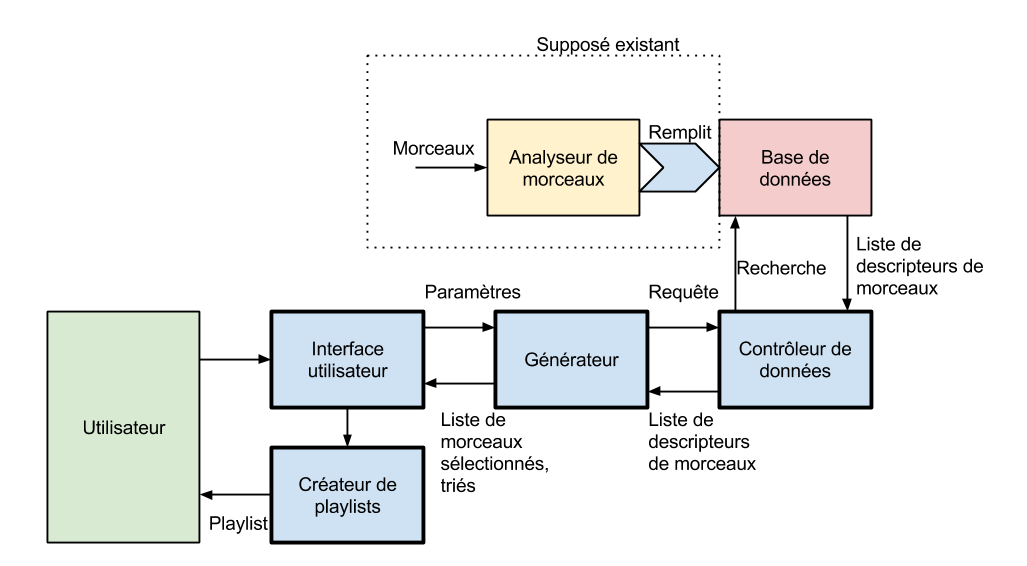
\includegraphics[width=14cm]{modules.png}
\caption{Les 4 modules indispensables au bon fonctionnement du programme et leurs
interactions.}
\end{figure}

\subsection{Ergonomie}
\label{besoins:nfonc:perf:erg}
Les interfaces utilisateurs devront être utilisables par un utilisateur
non-avancé, être claires et précises, et éviter de perdre l’utilisateur. Les
termes employés sur cette interface devront être écrit dans un vocabulaire
compréhensible de tous.
